\documentclass[11pt,a4paper]{ivoa}
\input tthdefs

% suggestions by Mireille tagged as %mir

%mir \title{Mango: A Component and Association Based Model for Source Data}
\title{Mango: A Component and Association Based Model for representing data for astronomical sources}

% see ivoatexDoc for what group names to use here
\ivoagroup{DM}


\author{François Bonnarel}
\author{Gilles Landais}
\author{Laurent Michel}
\author{Jesus Salgado}
\author{Mireille Louys}
\author{Marco Molinaro}

\editor{Laurent Michel}

% \previousversion[????URL????]{????Concise Document Label????}
\previousversion{This is the first public release}
%mir 
\today

\begin{document}
\begin{abstract}
The Mango model proposes a flexible way to expose data related to astronomical source objects in an interoperable way. (petite modif pour tester)
It takes into account the huge diversity of source data in terms of feature description, format and usage. 
The Mango model attaches an identifier on an astronomical source and associates to it all data related : observed physical quantities called parameters in this context, and other information like spectra, time series, preview image, etc ... for that source. 
Parameters usually appear in the columns of a source catalogue. Additionnal dataproducts are bound to the source to contribute to the science analysis and enhance data understanding.

Parameters are modeled by the IVOA MCT DM reusing both native and extended classes. Parameters' roles are given by UCDs and semantic tags.
Associated data can be simple URLs, VO service endpoints or VO data model instances. Their roles are also qualified by semantic tags.

\end{abstract}


\section*{Acknowledgments}

We would like to thank all those who took the time to present their own use cases (INAF, CDS, CFA, ESAC) on which the model has been built.

We would also like to thank all the people having tested Mango on their own data.


We would like to thank all those who took the time to present their own use cases (INAF, CDS, CFA, ESAC) on which the model has been built.
We would also like to thank all the people having tested Mango on their own data.

\section*{Model Name}
This model was initially named with a very explicit but hard to remember acronym, \texttt{CAB-MSD} standing for Component and Association Based Model for Source Data. We decided later to rename it \texttt{Mango} with reference to the inside out mango picture used to introduce the model in Groningen. As the tradition requires that such unexpected names are acronyms, let's assume that \texttt{Mango} stands for Model for ANnotating Generic Objects.


\section*{Conformance-related definitions}

The words ``MUST'', ``SHALL'', ``SHOULD'', ``MAY'', ``RECOMMENDED'', and
``OPTIONAL'' (in upper or lower case) used in this document are to be
interpreted as described in IETF standard RFC2119 \citep{std:RFC2119}.

The \emph{Virtual Observatory (VO)} is a
general term for a collection of federated resources that can be used
to conduct astronomical research, education, and outreach.
The \href{http://www.ivoa.net}{International
Virtual Observatory Alliance (IVOA)} is a global
collaboration of separately funded projects to develop standards and
infrastructure that enable VO applications.


\section{Introduction}

The source DM is a long term concern for the DM working group and more generally for the IVOA.
In the past years, there were some proposals to design a global model for sources \citep{wd:jesusdm} of for catalogs \citep{wd:catalog}.
Other proposals, more model-agnostic, were focused on the data annotation in VOTables \citep{note:stcvot} \citep{note:seb}. In this case the goal was no longer to design a source model but to provide a complete description of  individual quantities (positions, velocity…).
None of these proposals have come to completion

The source DM issue resurfaced at the spring 2018 Interop in Victoria during an hands-on session focused on the tools available to work with VO data models and especially with VO-DML. The goal of this session was to annotate data from different origins in order to make them interoperable with each other. The main concern expressed during this session was not related to the tools themselves but to the lack of models for sources. 
This is a big paradox in the VO world ; source data which represent the basic bricks of the astronomer work, have no model. This paradox can be explained by the fact that sources data are multifaceted. The way of which source data are organized depends on the survey they come from, one the way they have been generated  and on the expected use. In a more general way, it depends on the science we want to do with them. This diversity cannot be endorsed by a single model. Having a global source model would lead to a very complex solution not usable in practice.

This standard proposes to overcome this paradox presenting model based on independent components and associated data that can be embedded on demand in a container.

\emph{Not designed to describe what a source is nut to help clients to discover and to understand the quantities available for a particular source instance TBC}

\subsection{Role within the VO Architecture}

\begin{figure}
\centering

% As of ivoatex 1.2, the architecture diagram is generated by ivoatex in
% SVG; copy ivoatex/archdiag-full.xml to archdiag.xml and throw out
% all lines not relevant to your standard.
% Notes don't generally need this.  If you don't copy archdiag.xml,
% you must remove archdiag.svg from FIGURES in the Makefile.

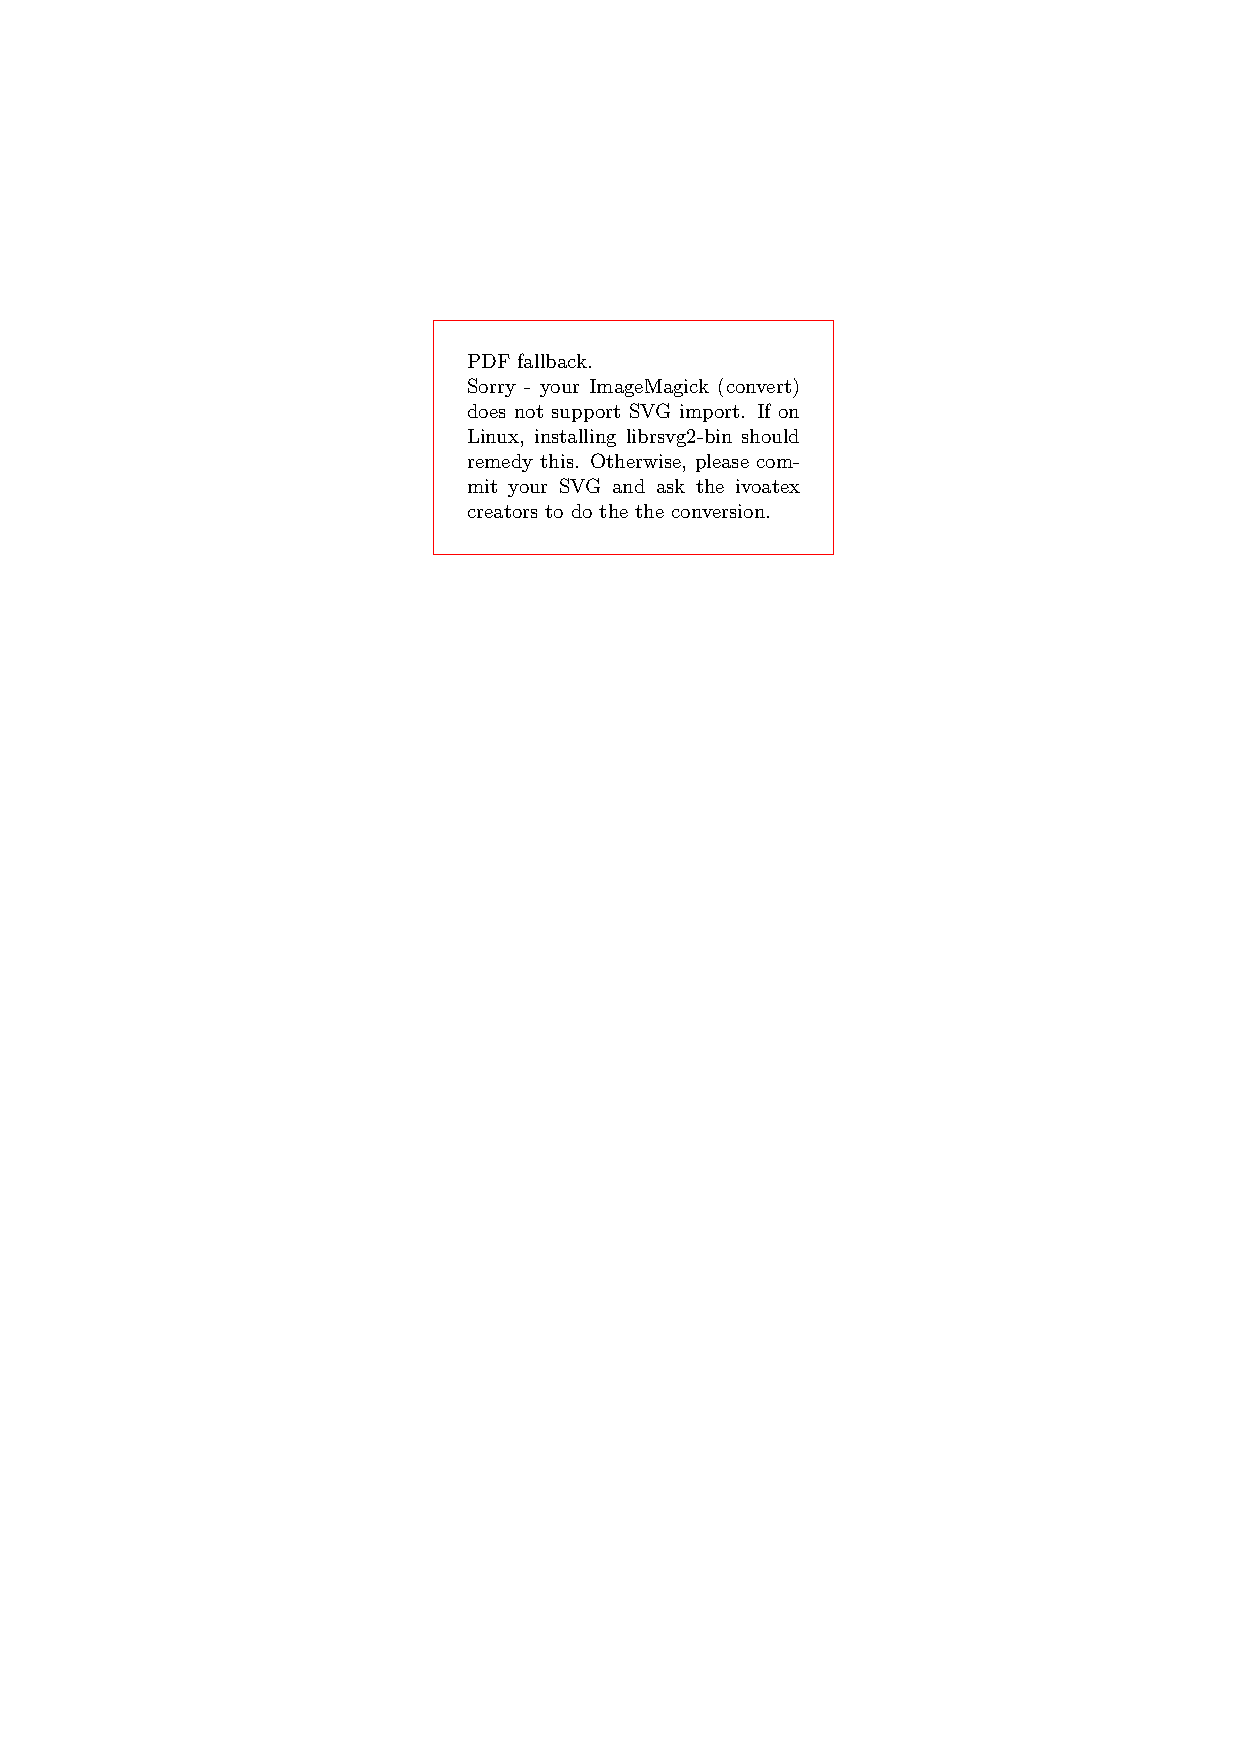
\includegraphics[width=0.9\textwidth]{role_diagram.pdf}
\caption{Architecture diagram for this document}
\label{fig:archdiag}
\end{figure}

Fig.~\ref{fig:archdiag} shows the role this document plays within the
IVOA architecture \citep{note:VOARCH}.



\section{Use Cases and  Requirements}

\subsection{Use Cases}
The use case below have been collected in 2019 from representative of some missions, archive or tools. The contribution was totally open. This gave a good picture of the needs but it's safe to say that not everything will supported by this first version.

\subsubsection{Gaia}
\begin{itemize}
    \item identifier
    \item reference position
    \item proper motion
    \item parallax and distance
    \item correlation,
    \item source extension
    \item radial velocity
    \item redshift
    \item luminosity
    \item date
    \item multiple detection
\end{itemize}


\subsubsection{Euclid}
\begin{itemize}    
    \item identifier
    \item position
    \item correlation with Gaia
    \item photometry (ground + sat),
    \item morphology
    \item redshift
    \item photometric redshift
\end{itemize}

\subsubsection{Exoplanets}
\begin{itemize}
    \item position
    \item orbit
    \item different source level(star, planet, moon)
    \item status and classification
    \item orbiting system description
\end{itemize}

\subsubsection{Morphologically Complex Structures}
\begin{itemize}    
    \item morphology
\end{itemize}

\subsubsection{Chandra} 
All quantities are time dependant,
Dependant on calibration + physical
model
\begin{itemize}    
    \item name
    \item pos
    \item time
    \item extension
    \item PHA 
\end{itemize}

\subsubsection{Vizier} 
All possible measure are present in Vizier in addition to lots of associated data 
\begin{itemize}    
    \item pre-existing data
    \item grouping columns
    \item lots of available metadata
    \item column name formatting
    \item one column different frames
\end{itemize}

\subsubsection{Aladin}

Quantities possibly plotted or matched with some of other datasets
\begin{itemize}
    \item position
    \item time
    \item flux
    \item link
    \item FoV
    \item column grouping
\end{itemize}

\subsubsection{X\-match}
\begin{itemize}
    \item Identifier
    \item position
    \item proper motion
    \item photometry
\end{itemize}

\subsubsection{Time Domain}
\begin{itemize}
    \item Identifier: object identifier
    \item Position: moving object
    \item Associated products: time series of e.g. a spectrum or an image
    \item Photometry: for light curves
    \item Timestamp: Independent axis of the time series
\end{itemize}

There are 2 distinct categories of requested quantities , the measures and the associated data. The measures
 can be numerical values or simple strings. The Mango measures rely on the Meas model. The associated data are related to data with a complex structures or to references. table  \ref{tab:q_breakup} shows the breaking up of the quantities liste above in these 2 categories

\begin{table}[ht!]
     \tiny
     \begin{tabular}{|p{2.4cm}|p{0.4cm}|p{0.4cm}|p{0.4cm}|p{0.6cm}|p{0.4cm}|p{0.4cm}|p{0.4cm}|p{0.4cm}|p{0.4cm}|}
       \hline Quantity &  Ga &  Eu &  Ex &  MCS  &  Ch&  Vi &  Al &  Xm&  TD \\
       \hline  \texttt{identifier}      &  p & P  &P& &P&P &P&  & P \\              
       \hline  \texttt{position}      &  p & P  &P& &P&P &P&  & P \\       
       \hline  \texttt{pr. motion}   & p &   &   &    &  &   &P&P&    \\       
       \hline  \texttt{distance}     & p &   &   &    &  &   &P&  &    \\       
       \hline  \texttt{correlation}   & AD &AD&   &    &  &AD &   &  &    \\       
       \hline  \texttt{extension}     &P&   &P&P &P&P& P&  &    \\       
       \hline  \texttt{rad. vel.}       &  P &   &   &    &  &P&   &  &    \\       
       \hline  \texttt{redshift}        &  P &P&   &    &  &P&   &  &    \\             
       \hline  \texttt{phot. rsft}      &   &P&   &    &  &P&   &  &    \\       
       \hline  \texttt{luminosity}    & P&P&   &    &  &P&P&P&P\\       
       \hline  \texttt{date}             & P  &   &   &    & P&P&   &  &P\\       
       \hline  \texttt{detections}    &  AD &   &   &    &  &   &   &  &    \\       
       \hline  \texttt{orbit}             &   &   &P& &  &   &   &  &    \\       
       \hline  \texttt{type}             &   &   & P& &  &P&   &  &    \\      
       \hline  \texttt{status}          &   &   &   &    &  &P&   &  &    \\       
       \hline  \texttt{orb. sys.}      &   &   &  P &    &  &   &   &  &    \\       
       \hline  \texttt{PHA}            &   &   &   &    &P&   &   &  &    \\       
       \hline  \texttt{ass. prd.}     &   &   &   &    &  &AD&   &  &AD \\       
       \hline 
     \end{tabular}
     \caption{ Break up of the requested quantities \texttt{P} parameter, \texttt{AD} Associated data} 
     \label{tab:q_breakup}
 \end{table}


\subsection{Requirements}

\subsubsection{R01: Supported Quantities}
\begin{itemize}
    \item Mango must provide unique source identifiers.
    \item Mango must provide modeling classes for both parameters and associated data.
    \item The number of parameters attached to Mango instances must be free.
    \item The number of associated data attached to Mango instances must be free.
\end{itemize}

\subsubsection{R02: Parameters}
The notion of parameter matches the concept of measure in the Meas model. Mango may support parameter classes that are not  Meas classes though.
  
\begin{itemize}
    \item Mango must support explict classes for the most used parameters.
    \item Mang must provide a generic way to support parameters that have not specif classes.
    \item Mango instances must support multiple instances of the same parameter class.
    \item The presence of any parameter in Mango instances must be optional.
    \item Mango must provide a way to identify the role of each parameter.
    \item The role of each parameter should be machine-readable.
    \item Each parameter must be able to be attached to a timestamp or a flag. The meaning of these flag is not part of Mango, but Mango must provide a way to describe it.
\end{itemize}

\subsubsection{R03: Associated Data}
The notion of associated data relates to any sort of complex data. This can be a pointer to a service or a data set, a data table or  other data structure.
\begin{itemize}
    \item Mango must support references to external datasets.
    \item Mango must support references to external services.
    \item Mango must support references to other Mango instances.
    \item Mango  must support references to instances of models serialized in VO-DML. 
    \item Mango instances must support multiple instances of the same associated data class.
    \item The presence of any associated data in Mango instances must be optional.
    \item Mango must provide a way to identify the role of each associated data.
    \item The role of each associated data should be machine-readable.
 \end{itemize}

\section{Model Overview}

\begin{figure}
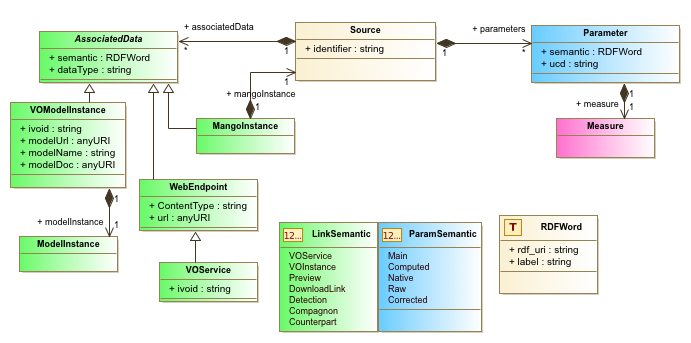
\includegraphics[width=0.9\textwidth]{../model/overview_diagram.png}
\caption{Mango overview}
\label{fig:overview}
\end{figure}

The root class of the model is the \texttt{Source} class that has only one attribute, the identifier, that is the only quantity common to  all  Mango instances.

Each quantity or associated data attached to a source is represented by a connector describing the nature of either the quantity or of the associated data.

There is no restriction on the set of connectors attached to one source.
There are 2 classes of connectors

\subsection{The parameters} 
Parameter connectors are used to bind measures with the source. One connector can only reference one measure. The measure itself is modeled by a class of the Measure model or by an extension of this model. Measure extensions are part of Mango. 
In addition to its class, the nature of a measure is given by a UCD and a semantic tag. The UCD gives the physical meaning of the measure whereas the semantic tag says more about the usage context of the measure. This can be for instance the reduction status (raw, corrected). The vocabulary allowed for the semantic is managed as a VO vocabulary. 


\begin{table}[ht!]
     \tiny
     \begin{tabular}{|p{2.4cm}|p{1.8cm}|p{7cm}|}
       \hline Quantity &  Model &  \\
       \hline  \texttt{identifier}      & Mango & required for anu instance\\                    
       \hline  \texttt{position}      &  Meas &  \\       
       \hline  \texttt{pr. motion}   & Meas &     \\       
       \hline  \texttt{distance}     & Ext Meas &     \\       
       \hline  \texttt{correlation}   & Ass data & reference to other Mango instances     \\       
       \hline  \texttt{extension}     & Ext Meas & Can be used for FoV, morphlogy or shape\\       
       \hline  \texttt{rad. vel.}       &  Ext Meas  &       \\       
       \hline  \texttt{redshift}        &   Ext Meas  &  \\             
       \hline  \texttt{phot. rsft}      & Ext Meas&    \\       
       \hline  \texttt{luminosity}    & Ext Meas&\\       
       \hline  \texttt{date}             & Meas & date or time stamp\\       
       \hline  \texttt{detections}    & Ass data & reference to other Mango instances   \\       
       \hline  \texttt{orbit}             & Ext Meas&      \\       
       \hline  \texttt{type}             &Ext Meas&     \\      
       \hline  \texttt{status}          &Ext Meas&     \\       
       \hline  \texttt{orb. sys.}      &Ext Meas&     \\       
       \hline  \texttt{PHA}            &Ext Meas&     \\       
       \hline  \texttt{ass. prd.}     &Ass data&  \\       
       \hline 
     \end{tabular}
     \caption{ \texttt{Meas} Measue class, \texttt{Ext Meas } Measure extension, \texttt{Ass data  } Mangno associated data} 
 \end{table}


\subsubsection{Parameter UCD}

\begin{table}[ht!]
     \begin{tabular}{|p{4cm}|p{3cm}|p{3.5cm}|}
       \hline Parameter &  Original model & UCDs 1+ first word  \\
       \hline  \texttt{Position}             &  Measure  &  pos \\       
       \hline  \texttt{Velocity  }            &  Measure & phys.veloc      \\              
       \hline  \texttt{Proper motion}    & Measure & pos.pm    \\       
       \hline  \texttt{Time}                   & Measure &  time.epoch   \\       
       \hline  \texttt{Polarization}         & Measure & phys.polarization \\      
       \hline  \texttt{SphericalSkyPosition}    &  Mango  &  pos.eq \\       
       \hline  \texttt{ObjectType}                   &  Mango  & src.class \\       
       \hline  \texttt{Redshift}                        &  Mango  & src.redshift \\       
       \hline  \texttt{Luminosity}                    &  Mango  & phot.qqqchose \\
       \hline  \texttt{HardnessRatio}             &  Mango  & phot.flux;arith.ratio \\
       \hline  \texttt{Shape}                     &  Mango  & phys.area \\
       \hline  \texttt{Flag}                        &  Mango  & meta.code  \\
       \hline  \texttt{Orbit}                       &  Mango  & src.orbital \\    
       \hline  \texttt{GenericMeasure}    &  Measure  &  Appropiate physical UCD \\    
       \hline 
     \end{tabular}
     \caption{ UCDs to be set for the supported parameters} 
     \label{tab:ucds}
 \end{table}

TBC phys.luminosity  vs phot.flux
ajoutdr une temperature

\subsection{Associated Data} 
Associated data connectors are used to bind any sort of complex data with the source. One connector can only refer to one dataset. Associated data can be either URIs (VO services or not) or reference to instances of other VO models (Obscore, Provenance…).

Attaching VO model instances to sources does not mean that these  models must be imported. The merge between a Mango instance and one associated instance is operated by the data annotation process. The indication given by Mango tell the client how to interpret the embedded instance

\subsection{STC Extension} 

All STC measures are built upon the same pattern (see fig \ref{fig:stcpattern}). The value(s) \texttt{Measure} object is carried by a \texttt{Coordinate} object. The coordinate is attached to a system (class \texttt{CoordSys}). The system has 2 components 1) the space  (class \texttt{CoordSpace}) that describes the axis and 2) the frame    \texttt{CoordFrame}).  All Mango parameters are based on this pattern. Native STC classes are used when possible. Others parameters are built by extending STC classes . Figure \ref{fig:stcpattern}) shows the extended STC classes being part of Mango 
\begin{figure}
     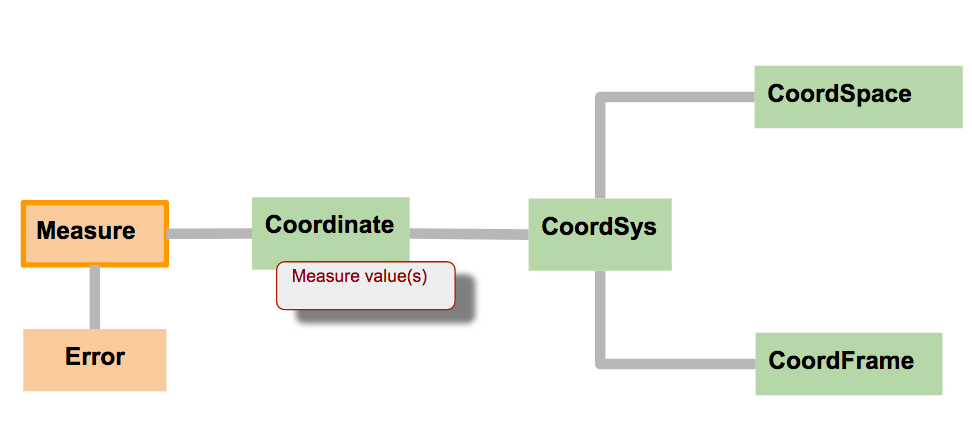
\includegraphics[width=0.9\textwidth]{stc_pattern.png}
     \caption{STC pattern (simplified view)}
     \label{fig:stcpattern}
\end{figure}

\begin{figure}
  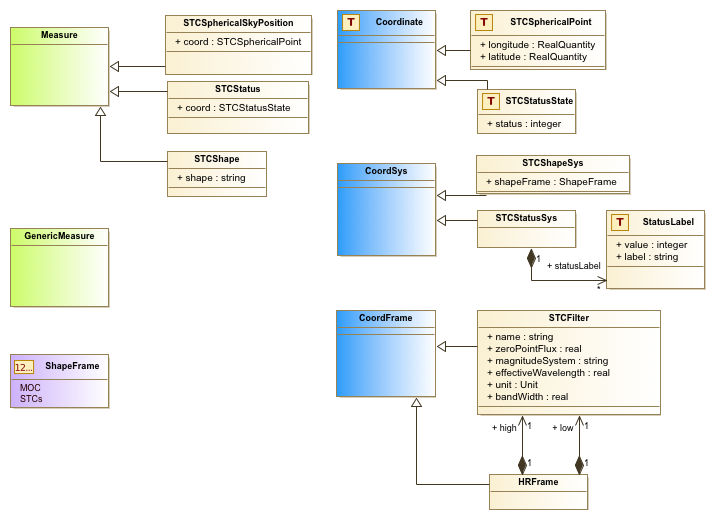
\includegraphics[angle=90,origin=c,width=1\textwidth]{../model/stc_ext_diagram.png}
  \caption{STC extension diagram }
  \label{fig:stcextension}
\end{figure}



% -------------------------------------------
% Items to substitute into the ivoatex document template.
%
%\ivoagroup{Data Model Working Group}

%\title{Mango}


%\author{Laurent Michel}
    
%\author{François Bonnarel}
    
%\author{Gilles Landais}
    
%\author{Mireille Louys}
    
%\author{Marco Molinaro}
    
%\author{Jesue Salgado}
    
%\previousversion{0.0}
      
% -------------------------------------------

\pagebreak
\section{Model: mango }
  
  % INSERT FIGURE HERE
  %\begin{figure}[h]
  %\begin{center}
  %  \includegraphics[width=\textwidth]{????.png}
  %  \caption{???}\label{fig:????}
  %\end{center}
  %\end{figure}

  Data model based oon components and data association for source data

  \subsection{AssociatedData (Abstract)}
  \label{sect:AssociatedData}
    Abstract reference to a particular dataset associated to the Source. This class is used to specify the type of the dataset as well as its role.

    \subsubsection{AssociatedData.semantic}
      \textbf{vodml-id: AssociatedData.semantic} \newline
      \textbf{type: \hyperref[sect:stcextend.RDFWord]{mango:stcextend.RDFWord}} \newline
      \textbf{multiplicity: 1} \newline 
      Reference to a semantic concept giving the nature of the associated data. As long as the vocabulary is not set, the possible values of this attribute are given by the LinkSemantic enumeration.

    \subsubsection{AssociatedData.dataType}
      \textbf{vodml-id: AssociatedData.dataType} \newline
      \textbf{type: \hyperref[sect:ivoa]{ivoa:string}} \newline
      \textbf{multiplicity: 1} \newline 
      Type of the associated data (not defined yet)

    \subsubsection{AssociatedData.description}
      \textbf{vodml-id: AssociatedData.description} \newline
      \textbf{type: \hyperref[sect:ivoa]{ivoa:string}} \newline
      \textbf{multiplicity: 1} \newline 
      Free text description of the associated data

  \subsection{HardnessRatioSys}
  \label{sect:HardnessRatioSys}
    TODO : Missing description : please, update your UML model asap.

    \noindent \textbf{subset} \newline
    \indent   \textbf{role: coords:PhysicalCoordSys.frame} \newline
    \indent   \textbf{type: mango:HRFrame} \newline


  \subsection{MangoInstance}
  \label{sect:MangoInstance}
    Reference to another CAB-MSD instance that is part of the associated data.

    \subsubsection{MangoInstance.mangoInstance}
      \textbf{vodml-id: MangoInstance.mangoInstance} \newline
      \textbf{type: \hyperref[sect:Source]{mango:Source}} \newline
      \textbf{multiplicity: 1} \newline 
      Composition link pointing on one cab\_msd instance associated with the source.

  \subsection{ModelInstance}
  \label{sect:ModelInstance}
    Placeholder for the mapping of the model instance

  \subsection{Parameter}
  \label{sect:Parameter}
    Reference to a particular measure of the Source. This class is used to specify the type of the measure as well as its role.

    \noindent \textbf{constraint} \newline
    \indent    \textbf{detail: Parameter.One association at the time
 }\newline


    \subsubsection{Parameter.semantic}
      \textbf{vodml-id: Parameter.semantic} \newline
      \textbf{type: \hyperref[sect:stcextend.RDFWord]{mango:stcextend.RDFWord}} \newline
      \textbf{multiplicity: 1} \newline 
      Reference to a semantic concept giving the nature of the parameter As long as the vocabulary is not set, the possible values of this attribute are given by the ParamSemantic enumeration.

    \subsubsection{Parameter.ucd}
      \textbf{vodml-id: Parameter.ucd} \newline
      \textbf{type: \hyperref[sect:ivoa]{ivoa:string}} \newline
      \textbf{multiplicity: 1} \newline 
      UCD1+ giving the type of the physical measure

    \subsubsection{Parameter.description}
      \textbf{vodml-id: Parameter.description} \newline
      \textbf{type: \hyperref[sect:ivoa]{ivoa:string}} \newline
      \textbf{multiplicity: 1} \newline 
      Free text description of the measure

    \subsubsection{Parameter.measure}
      \textbf{vodml-id: Parameter.measure} \newline
      \textbf{type: meas:Measure} \newline
      \textbf{multiplicity: 1} \newline 
      Composition link pointing to the meas:Measure instance

    \subsubsection{Parameter.associatedParameters}
      \textbf{vodml-id: Parameter.associatedParameters} \newline
      \textbf{type: \hyperref[sect:Parameter]{mango:Parameter}} \newline
      \textbf{multiplicity: 0..*} \newline 
      TODO : Missing description : please, update your UML model asap.

  \subsection{PhotometryCoordSys}
  \label{sect:PhotometryCoordSys}
    TODO : Missing description : please, update your UML model asap.

    \noindent \textbf{subset} \newline
    \indent   \textbf{role: coords:PhysicalCoordSys.frame} \newline
    \indent   \textbf{type: mango:PhotFilter} \newline


  \subsection{Source}
  \label{sect:Source}
    Root class of the model. CAB\_MSF instance are meant ot be Source instances. A source ha an identifier and to sets of hooks: one for the parameters and one for the associated data.

    \subsubsection{Source.identifier}
      \textbf{vodml-id: Source.identifier} \newline
      \textbf{type: \hyperref[sect:ivoa]{ivoa:string}} \newline
      \textbf{multiplicity: 1} \newline 
      Unique identifier for a Source. The uniqness of that identifier is not managed by the model. The format is free.

    \subsubsection{Source.associatedData}
      \textbf{vodml-id: Source.associatedData} \newline
      \textbf{type: \hyperref[sect:AssociatedData]{mango:AssociatedData}} \newline
      \textbf{multiplicity: 0..*} \newline 
      Composition link pointing on all data associated with the source.

    \subsubsection{Source.parameters}
      \textbf{vodml-id: Source.parameters} \newline
      \textbf{type: \hyperref[sect:Parameter]{mango:Parameter}} \newline
      \textbf{multiplicity: 0..*} \newline 
      Composition link pointing on all parameters attached to the source.

  \subsection{Temperature}
  \label{sect:Temperature}
    TODO : Missing description : please, update your UML model asap.

    \subsubsection{Temperature.coord}
      \textbf{vodml-id: Temperature.coord} \newline
      \textbf{type: \hyperref[sect:ivoa]{ivoa:string}} \newline
      \textbf{multiplicity: 1} \newline 
      TODO : Missing description : please, update your UML model asap.

  \subsection{VOModelInstance}
  \label{sect:VOModelInstance}
    Reference to a VO model instance that is part of the associated data.

    \subsubsection{VOModelInstance.ivoid}
      \textbf{vodml-id: VOModelInstance.ivoid} \newline
      \textbf{type: \hyperref[sect:ivoa]{ivoa:string}} \newline
      \textbf{multiplicity: 1} \newline 
      VO-DML id of the referenced model

    \subsubsection{VOModelInstance.modelUrl}
      \textbf{vodml-id: VOModelInstance.modelUrl} \newline
      \textbf{type: \hyperref[sect:ivoa]{ivoa:anyURI}} \newline
      \textbf{multiplicity: 1} \newline 
      URL on the VO-DML model

    \subsubsection{VOModelInstance.modelName}
      \textbf{vodml-id: VOModelInstance.modelName} \newline
      \textbf{type: \hyperref[sect:ivoa]{ivoa:string}} \newline
      \textbf{multiplicity: 1} \newline 
      Name of the referenced model

    \subsubsection{VOModelInstance.modelDoc}
      \textbf{vodml-id: VOModelInstance.modelDoc} \newline
      \textbf{type: \hyperref[sect:ivoa]{ivoa:anyURI}} \newline
      \textbf{multiplicity: 1} \newline 
      Documentation URL of the model

    \subsubsection{VOModelInstance.modelInstance}
      \textbf{vodml-id: VOModelInstance.modelInstance} \newline
      \textbf{type: \hyperref[sect:ModelInstance]{mango:ModelInstance}} \newline
      \textbf{multiplicity: 1} \newline 
      Composition link pointing on one VO instance instance associated with the source.

  \subsection{VOService}
  \label{sect:VOService}
    Class for associated data referenced by an URL that is a VO service

    \subsubsection{VOService.ivoid}
      \textbf{vodml-id: VOService.ivoid} \newline
      \textbf{type: \hyperref[sect:ivoa]{ivoa:string}} \newline
      \textbf{multiplicity: 1} \newline 
      IVOA id attached to the URI

  \subsection{WebEndpoint}
  \label{sect:WebEndpoint}
    Class for associated data referenced by an URL

    \subsubsection{WebEndpoint.ContentType}
      \textbf{vodml-id: WebEndpoint.ContentType} \newline
      \textbf{type: \hyperref[sect:ivoa]{ivoa:string}} \newline
      \textbf{multiplicity: 1} \newline 
      Mime type of the URL

    \subsubsection{WebEndpoint.url}
      \textbf{vodml-id: WebEndpoint.url} \newline
      \textbf{type: \hyperref[sect:ivoa]{ivoa:anyURI}} \newline
      \textbf{multiplicity: 1} \newline 
      Web endpoint

  \subsection{LinkSemantic}
  \label{sect:LinkSemantic}

  Literal enumeration of the possible values for the associated data semantic. This stands for an example before we have defined a vocabulary.

  \noindent \underline{Enumeration Literals}
  \vspace{-\parsep}
  \small
  \begin{itemize}
  
    \item[\textbf{VOService}]: \textbf{vodml-id:} LinkSemantic.VOService \newline
          \textbf{description:} Data returned by a VO service
    \item[\textbf{VOInstance}]: \textbf{vodml-id:} LinkSemantic.VOInstance \newline
          \textbf{description:} Data Serialized in a VO model
    \item[\textbf{Preview}]: \textbf{vodml-id:} LinkSemantic.Preview \newline
          \textbf{description:} data preview
    \item[\textbf{DownloadLink}]: \textbf{vodml-id:} LinkSemantic.DownloadLink \newline
          \textbf{description:} Data download link
    \item[\textbf{Detection}]: \textbf{vodml-id:} LinkSemantic.Detection \newline
          \textbf{description:} Particular detection
    \item[\textbf{Compagnon}]: \textbf{vodml-id:} LinkSemantic.Compagnon \newline
          \textbf{description:} Compagnon source
    \item[\textbf{Counterpart}]: \textbf{vodml-id:} LinkSemantic.Counterpart \newline
          \textbf{description:} Counter part source
  \end{itemize}
  \normalsize


  \subsection{ParamSemantic}
  \label{sect:ParamSemantic}

  Literal enumeration of the possible values for the parameter semantic. This stands for an example before we have defined a vocabulary.

  \noindent \underline{Enumeration Literals}
  \vspace{-\parsep}
  \small
  \begin{itemize}
  
    \item[\textbf{Main}]: \textbf{vodml-id:} ParamSemantic.Main \newline
          \textbf{description:} Main measurment
    \item[\textbf{Computed}]: \textbf{vodml-id:} ParamSemantic.Computed \newline
          \textbf{description:} Computed measurement
    \item[\textbf{Native}]: \textbf{vodml-id:} ParamSemantic.Native \newline
          \textbf{description:} Mative measurement
    \item[\textbf{Raw}]: \textbf{vodml-id:} ParamSemantic.Raw \newline
          \textbf{description:} raw measure
    \item[\textbf{Corrected}]: \textbf{vodml-id:} ParamSemantic.Corrected \newline
          \textbf{description:} Corrected measure
  \end{itemize}
  \normalsize


\pagebreak
\section{Package: stcextend }

  % INSERT FIGURE HERE
  %\begin{figure}[h]
  %\begin{center}
  %  \includegraphics[width=\textwidth]{????.png}
  %  \caption{???}\label{fig:????}
  %\end{center}
  %\end{figure}

  This package contains all object and type classes that has been extended from the Measure and Coordinates models. This extension mechanism is used to add new types of measures while staying whithin the Mes/Coords pattern.

  \subsection{Flag}
  \label{sect:stcextend.Flag}
    Measure to be used for status parameters

    \subsubsection{Flag.coord}
      \textbf{vodml-id: stcextend.Flag.coord} \newline
      \textbf{type: \hyperref[sect:stcextend.FlagCoord]{mango:stcextend.FlagCoord}} \newline
      \textbf{multiplicity: 1} \newline 
      Coordinate holding the statsu value

  \subsection{FlagCoord}
  \label{sect:stcextend.FlagCoord}
    Coordinate of a status Measure

    \noindent \textbf{subset} \newline
    \indent   \textbf{role: coords:Coordinate.coordSys} \newline
    \indent   \textbf{type: FlagSys} \newline


    \subsubsection{FlagCoord.status}
      \textbf{vodml-id: stcextend.FlagCoord.status} \newline
      \textbf{type: \hyperref[sect:ivoa]{ivoa:integer}} \newline
      \textbf{multiplicity: 1} \newline 
      Value of the status

  \subsection{FlagState}
  \label{sect:stcextend.FlagState}
    Possible value of a status

    \subsubsection{FlagState.value}
      \textbf{vodml-id: stcextend.FlagState.value} \newline
      \textbf{type: \hyperref[sect:ivoa]{ivoa:integer}} \newline
      \textbf{multiplicity: 1} \newline 
      Status value

    \subsubsection{FlagState.label}
      \textbf{vodml-id: stcextend.FlagState.label} \newline
      \textbf{type: \hyperref[sect:ivoa]{ivoa:string}} \newline
      \textbf{multiplicity: 1} \newline 
      Label attached to that status value

  \subsection{FlagSys}
  \label{sect:stcextend.FlagSys}
    Coordinate system to be used for statur measures.

    \subsubsection{FlagSys.statusLabel}
      \textbf{vodml-id: stcextend.FlagSys.statusLabel} \newline
      \textbf{type: \hyperref[sect:stcextend.FlagState]{mango:stcextend.FlagState}} \newline
      \textbf{multiplicity: 0..*} \newline 
      Composition loink to all possible status values for this system

  \subsection{HRFrame}
  \label{sect:stcextend.HRFrame}
    Hardness ratio frame. Defined by 2 energy bands Eheigh ELow. HR = (Eheigh - Elow)/(Eheigh + Elow) Energy bands are deemed to special photometric filters

    \subsubsection{HRFrame.low}
      \textbf{vodml-id: stcextend.HRFrame.low} \newline
      \textbf{type: \hyperref[sect:stcextend.PhotFilter]{mango:stcextend.PhotFilter}} \newline
      \textbf{multiplicity: 1} \newline 
      Low energy band

    \subsubsection{HRFrame.high}
      \textbf{vodml-id: stcextend.HRFrame.high} \newline
      \textbf{type: \hyperref[sect:stcextend.PhotFilter]{mango:stcextend.PhotFilter}} \newline
      \textbf{multiplicity: 1} \newline 
      Heigh energy band

  \subsection{HardnessRatio}
  \label{sect:stcextend.HardnessRatio}
    TODO : Missing description : please, update your UML model asap.

    \subsubsection{HardnessRatio.coord}
      \textbf{vodml-id: stcextend.HardnessRatio.coord} \newline
      \textbf{type: \hyperref[sect:stcextend.HardnessRatioCoord]{mango:stcextend.HardnessRatioCoord}} \newline
      \textbf{multiplicity: 1} \newline 
      TODO : Missing description : please, update your UML model asap.

  \subsection{HardnessRatioCoord}
  \label{sect:stcextend.HardnessRatioCoord}
    TODO : Missing description : please, update your UML model asap.

    \noindent \textbf{subset} \newline
    \indent   \textbf{role: coords:Coordinate.coordSys} \newline
    \indent   \textbf{type: mango:HardnessRatioSys} \newline


    \subsubsection{HardnessRatioCoord.hardnessRatio}
      \textbf{vodml-id: stcextend.HardnessRatioCoord.hardnessRatio} \newline
      \textbf{type: \hyperref[sect:ivoa]{ivoa:real}} \newline
      \textbf{multiplicity: 1} \newline 
      TODO : Missing description : please, update your UML model asap.

  \subsection{LonLatCoordSys}
  \label{sect:stcextend.LonLatCoordSys}
    TODO : Missing description : please, update your UML model asap.

    \noindent \textbf{subset} \newline
    \indent   \textbf{role: coords:PhysicalCoordSys.frame} \newline
    \indent   \textbf{type: coords:SpaceFrame} \newline


    \noindent \textbf{constraint} \newline
    \indent    \textbf{detail: LonLatCoordSys.coordSpace[0] }\newline


  \subsection{LonLatPoint}
  \label{sect:stcextend.LonLatPoint}
    Coordinate of a point on the sky sphere expressed in spherical coordinates.

    \noindent \textbf{subset} \newline
    \indent   \textbf{role: coords:Coordinate.coordSys} \newline
    \indent   \textbf{type: mango:LonLatCoordSys} \newline


    \subsubsection{LonLatPoint.longitude}
      \textbf{vodml-id: stcextend.LonLatPoint.longitude} \newline
      \textbf{type: \hyperref[sect:ivoa]{ivoa:real}} \newline
      \textbf{multiplicity: 1} \newline 
      longitude of the point

    \subsubsection{LonLatPoint.latitude}
      \textbf{vodml-id: stcextend.LonLatPoint.latitude} \newline
      \textbf{type: \hyperref[sect:ivoa]{ivoa:real}} \newline
      \textbf{multiplicity: 1} \newline 
      Latitude of the point

  \subsection{LonLatSkyPosition}
  \label{sect:stcextend.LonLatSkyPosition}
    Measure to used for sky points expressed with a spherical coordinate system

    \subsubsection{LonLatSkyPosition.coord}
      \textbf{vodml-id: stcextend.LonLatSkyPosition.coord} \newline
      \textbf{type: \hyperref[sect:stcextend.LonLatPoint]{mango:stcextend.LonLatPoint}} \newline
      \textbf{multiplicity: 1} \newline 
      Coordinate of spherical sky position

  \subsection{ObjectType}
  \label{sect:stcextend.ObjectType}
    TODO : Missing description : please, update your UML model asap.

    \subsubsection{ObjectType.coord}
      \textbf{vodml-id: stcextend.ObjectType.coord} \newline
      \textbf{type: \hyperref[sect:stcextend.OrbitCoord]{mango:stcextend.OrbitCoord}} \newline
      \textbf{multiplicity: 1} \newline 
      TODO : Missing description : please, update your UML model asap.

  \subsection{ObjectTypeCoord}
  \label{sect:stcextend.ObjectTypeCoord}
    TODO : Missing description : please, update your UML model asap.

    \noindent \textbf{subset} \newline
    \indent   \textbf{role: coords:Coordinate.coordSys} \newline
    \indent   \textbf{type: ObjectTypeSys} \newline


    \subsubsection{ObjectTypeCoord.objectType}
      \textbf{vodml-id: stcextend.ObjectTypeCoord.objectType} \newline
      \textbf{type: \hyperref[sect:ivoa]{ivoa:string}} \newline
      \textbf{multiplicity: 1} \newline 
      TODO : Missing description : please, update your UML model asap.

  \subsection{ObjectTypeSys}
  \label{sect:stcextend.ObjectTypeSys}
    TODO : Missing description : please, update your UML model asap.

  \subsection{Orbit}
  \label{sect:stcextend.Orbit}
    TODO : Missing description : please, update your UML model asap.

    \subsubsection{Orbit.coord}
      \textbf{vodml-id: stcextend.Orbit.coord} \newline
      \textbf{type: \hyperref[sect:stcextend.OrbitCoord]{mango:stcextend.OrbitCoord}} \newline
      \textbf{multiplicity: 1} \newline 
      TODO : Missing description : please, update your UML model asap.

  \subsection{OrbitCoord}
  \label{sect:stcextend.OrbitCoord}
    TODO : Missing description : please, update your UML model asap.

    \noindent \textbf{subset} \newline
    \indent   \textbf{role: coords:Coordinate.coordSys} \newline
    \indent   \textbf{type: coords:SpaceSys} \newline


  \subsection{PhotFilter}
  \label{sect:stcextend.PhotFilter}
    Photometric filter description, compliant with photDM

    \subsubsection{PhotFilter.name}
      \textbf{vodml-id: stcextend.PhotFilter.name} \newline
      \textbf{type: \hyperref[sect:ivoa]{ivoa:string}} \newline
      \textbf{multiplicity: 1} \newline 
      Filter name

    \subsubsection{PhotFilter.zeroPointFlux}
      \textbf{vodml-id: stcextend.PhotFilter.zeroPointFlux} \newline
      \textbf{type: \hyperref[sect:ivoa]{ivoa:real}} \newline
      \textbf{multiplicity: 1} \newline 
      Zero point flux of the filter

    \subsubsection{PhotFilter.magnitudeSystem}
      \textbf{vodml-id: stcextend.PhotFilter.magnitudeSystem} \newline
      \textbf{type: \hyperref[sect:ivoa]{ivoa:string}} \newline
      \textbf{multiplicity: 1} \newline 
      Magnitude system used by the filter

    \subsubsection{PhotFilter.effectiveWavelength}
      \textbf{vodml-id: stcextend.PhotFilter.effectiveWavelength} \newline
      \textbf{type: \hyperref[sect:ivoa]{ivoa:real}} \newline
      \textbf{multiplicity: 1} \newline 
      Effective wavelength of the filter

    \subsubsection{PhotFilter.unit}
      \textbf{vodml-id: stcextend.PhotFilter.unit} \newline
      \textbf{type: \hyperref[sect:ivoa]{ivoa:Unit}} \newline
      \textbf{multiplicity: 1} \newline 
      Wavelength unit used for that filter

    \subsubsection{PhotFilter.bandWidth}
      \textbf{vodml-id: stcextend.PhotFilter.bandWidth} \newline
      \textbf{type: \hyperref[sect:ivoa]{ivoa:real}} \newline
      \textbf{multiplicity: 1} \newline 
      Band width of the filter

  \subsection{Photometry}
  \label{sect:stcextend.Photometry}
    TODO : Missing description : please, update your UML model asap.

    \subsubsection{Photometry.coord}
      \textbf{vodml-id: stcextend.Photometry.coord} \newline
      \textbf{type: \hyperref[sect:stcextend.PhotometryCoord]{mango:stcextend.PhotometryCoord}} \newline
      \textbf{multiplicity: 1} \newline 
      TODO : Missing description : please, update your UML model asap.

  \subsection{PhotometryCoord}
  \label{sect:stcextend.PhotometryCoord}
    TODO : Missing description : please, update your UML model asap.

    \noindent \textbf{subset} \newline
    \indent   \textbf{role: coords:Coordinate.coordSys} \newline
    \indent   \textbf{type: PhotometryCoordSys} \newline


    \subsubsection{PhotometryCoord.luminosity}
      \textbf{vodml-id: stcextend.PhotometryCoord.luminosity} \newline
      \textbf{type: \hyperref[sect:ivoa]{ivoa:real}} \newline
      \textbf{multiplicity: 1} \newline 
      TODO : Missing description : please, update your UML model asap.

  \subsection{RDFWord}
  \label{sect:stcextend.RDFWord}
    Datatype for vocabulary word. Provides a pointer to the word description and a label.

    \subsubsection{RDFWord.rdf\_uri}
      \textbf{vodml-id: stcextend.RDFWord.rdf\_uri} \newline
      \textbf{type: \hyperref[sect:ivoa]{ivoa:string}} \newline
      \textbf{multiplicity: 1} \newline 
      URI extarcted from the DRF document and refering ot the word

    \subsubsection{RDFWord.label}
      \textbf{vodml-id: stcextend.RDFWord.label} \newline
      \textbf{type: \hyperref[sect:ivoa]{ivoa:string}} \newline
      \textbf{multiplicity: 1} \newline 
      RDF label. Matched the URL fragment for IVOA vocabularies

  \subsection{Redshift}
  \label{sect:stcextend.Redshift}
    TODO : Missing description : please, update your UML model asap.

    \subsubsection{Redshift.coord}
      \textbf{vodml-id: stcextend.Redshift.coord} \newline
      \textbf{type: \hyperref[sect:stcextend.RedshiftCoord]{mango:stcextend.RedshiftCoord}} \newline
      \textbf{multiplicity: 1} \newline 
      TODO : Missing description : please, update your UML model asap.

  \subsection{RedshiftCoord}
  \label{sect:stcextend.RedshiftCoord}
    TODO : Missing description : please, update your UML model asap.

    \noindent \textbf{subset} \newline
    \indent   \textbf{role: coords:Coordinate.coordSys} \newline
    \indent   \textbf{type: RedshiftSys} \newline


    \subsubsection{RedshiftCoord.redshift}
      \textbf{vodml-id: stcextend.RedshiftCoord.redshift} \newline
      \textbf{type: \hyperref[sect:ivoa]{ivoa:real}} \newline
      \textbf{multiplicity: 1} \newline 
      TODO : Missing description : please, update your UML model asap.

  \subsection{RedshiftSys}
  \label{sect:stcextend.RedshiftSys}
    TODO : Missing description : please, update your UML model asap.

  \subsection{Shape}
  \label{sect:stcextend.Shape}
    Measure giving the shape of a source

    \subsubsection{Shape.coord}
      \textbf{vodml-id: stcextend.Shape.coord} \newline
      \textbf{type: \hyperref[sect:stcextend.ShapeCoord]{mango:stcextend.ShapeCoord}} \newline
      \textbf{multiplicity: 1} \newline 
      String serialization of the source shape

  \subsection{ShapeCoord}
  \label{sect:stcextend.ShapeCoord}
    TODO : Missing description : please, update your UML model asap.

    \noindent \textbf{subset} \newline
    \indent   \textbf{role: coords:Coordinate.coordSys} \newline
    \indent   \textbf{type: ShapeSys} \newline


    \subsubsection{ShapeCoord.shape}
      \textbf{vodml-id: stcextend.ShapeCoord.shape} \newline
      \textbf{type: \hyperref[sect:ivoa]{ivoa:string}} \newline
      \textbf{multiplicity: 1} \newline 
      TODO : Missing description : please, update your UML model asap.

  \subsection{ShapeSys}
  \label{sect:stcextend.ShapeSys}
    Coordinate systen to be used for shape measure

    \subsubsection{ShapeSys.shapeFrame}
      \textbf{vodml-id: stcextend.ShapeSys.shapeFrame} \newline
      \textbf{type: \hyperref[sect:stcextend.ShapeFrame]{mango:stcextend.ShapeFrame}} \newline
      \textbf{multiplicity: 1} \newline 
      Frame of the shape measure. Gives a enumeration of the supported serializations.

  \subsection{ShapeFrame}
  \label{sect:stcextend.ShapeFrame}

  Enumeration of the possible options to encode a shape in a string.

  \noindent \underline{Enumeration Literals}
  \vspace{-\parsep}
  \small
  \begin{itemize}
  
    \item[\textbf{MOC}]: \textbf{vodml-id:} stcextend.ShapeFrame.MOC \newline
          \textbf{description:} MOC serialization
    \item[\textbf{STCs}]: \textbf{vodml-id:} stcextend.ShapeFrame.STCs \newline
          \textbf{description:} STCs serialization
  \end{itemize}
  \normalsize


\section{TAP and Mango}
This not normative section gives possible tips to save and discover Mango instances in TAP services.
We suppose that the TAP service hosts catalogs which sources are Mango instances. These catalogs are named \emph{Mango Catalogs}.

\subsection{Storing Mango Catalogs in TAP}
For now this section only concerns the parameter. The associated data will be taken into account later.

\begin{itemize}
  \item One master table for the catalogs with various meta-data out of the Mango scope plus a unique identifier (primary key)
  \item One master sources table for the source instances with the catalog identifier and a primary key safer than the Mango identifier.
  \item One table for each supported parameter with a foreign key for the join with the master source table
\end{itemize}

Although the model of the measures is hierarchical, it should be possible to flatten them in one single table considering that the model structure can be retrieved with the TAP\_SCHEMA annotations (TBC) 

This schema requires the server to explore all the parameter tables to retrieve  whole Mango instances. This process can be speed up by using the \emph{MangoCore} table.

\subsection{ \emph{MangoCore} Table}

The discovery of \emph{Mango Catalogs} can be helped by a  \emph{MangoCore} table located in the  \emph{schema} schema. As Mango is not dedicated to any specific domain, we cannot define a set of core parameters, but parameters can be flagged as \emph{Core Parameter}. This selection is left at the discretion of the curator.
The \emph{MangoCore} table has set of columns per parameter class plus one for the catalog ID. It has one row per stored catalog. Each parameter has at least 2 columns: one with the UCD an one with the \emph{Core} flag. TBC


\appendix
\section{Changes from Previous Versions}

No previous versions yet.  
% these would be subsections "Changes from v. WD-..."
% Use itemize environments.


% NOTE: IVOA recommendations must be cited from docrepo rather than ivoabib
% (REC entries there are for legacy documents only)
\bibliography{myrefs,ivoatex/ivoabib,ivoatex/docrepo}


\end{document}
